
\subsection{OpenStack ongoing extensions}
\label{subsec:ga_extensions}
\subsubsection{Trio2o and TriCircle} 
Tiro2o/TriCircle is an attempt to introduce scalability and manageability to a multi-site deployment of OpenStack by using the idea of API gateways. The core concepts of Trio2o/TriCircle are (1) an OpenStack deployment is divided into several sites where each site runs all key OpenStack services (2) Trio2o/TriCircle exposes a single OpenStack API endpoint to end-users giving them a view of a large (single) cloud with several availability zones that that represent the several sites  (3) Trio2o/TriCircle uses standard OpenStack APIs to communicate to the various OpenStack sites (see, e.g., Figure \ref{fig:Trio2oArch}). TriCircle and Trio2o together used to make up the OpenStack Cascading solution \cite{OpenStackCascading} until they were split back in 2016. When the split occurred, Trio2o was the project that dealt with the compute and storage aspects of things while TriCircle was the one that took care of the networking side of things. 

In the original design \cite{OpenStackCascading}, the solution was realized by a standard OpenStack instance that uses custom drivers for each service (e.g., a nova plugin in the top instance is capable managing the bottom instances through the nova-api interface). A similar concept is still used in TriCircle whereby  a custom plugin is used for Neutron at both the top and bottom OpenStack instances. On the other hand, Trio2o further simplifies the design by running unmodified OpenStack in the bottom sites while implementing  API gateways for Nova and Cinder as an advanced reverse proxy. In addition to the two gateways, Trio2o also includes an admin API for, e.g., AZ to region mapping and an Xjob service for any asynchronous job that may need to be executed in the background. In the current realization of these concepts, both Trio2o and TriCircle assume shared Keystone and Glance services while assuming sites are OpenStack regions that share these services.  

\begin{figure}[htbp]
\begin{center}
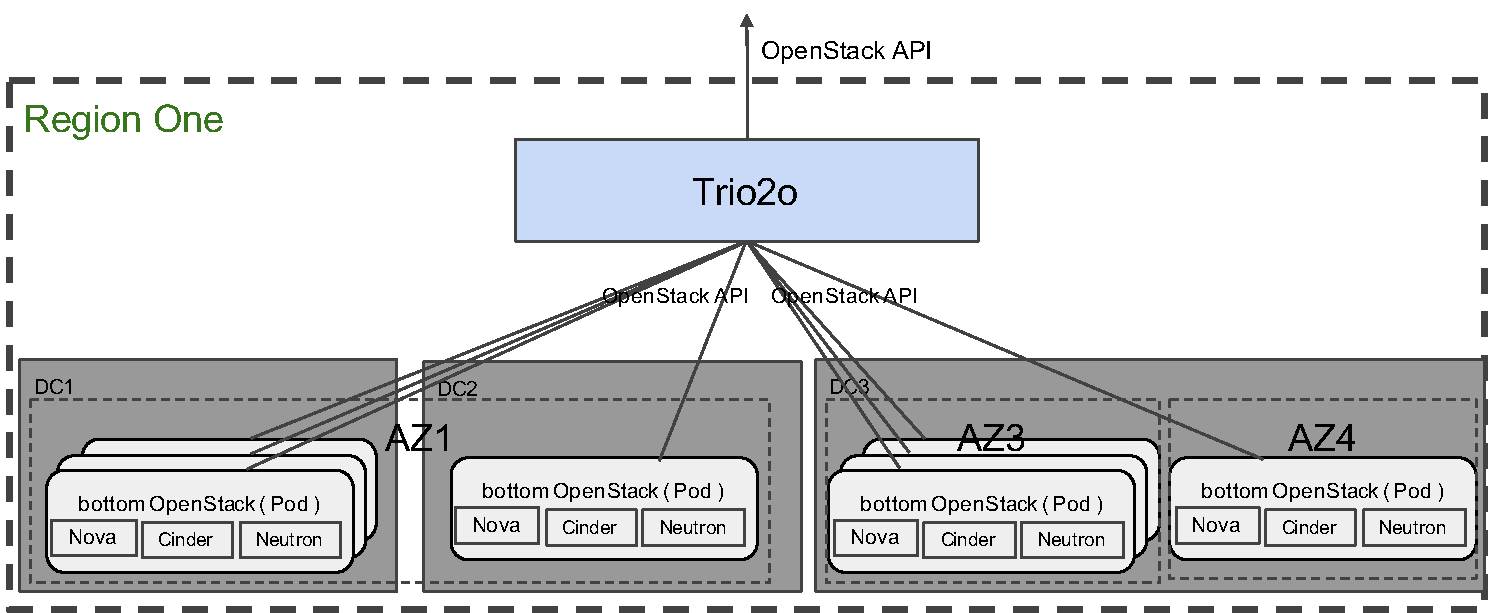
\includegraphics[width=0.5\textwidth]{trio2oarch}
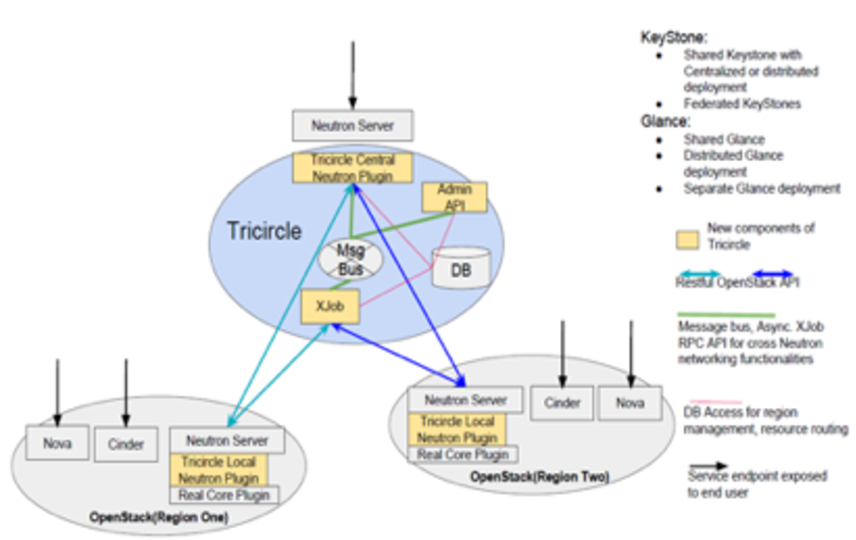
\includegraphics[width=0.5\textwidth]{tricirclearch}
\caption{High-level architecture of Trio2o \cite{Trio2oDesign} and TriCircle \cite{TriCircleDesign} }
\label{fig:Trio2oArch}
\end{center}
\end{figure}

Trio2o/Tricircle fulfills the requirements for Level 1 and 2. For level 3, a disconnected site will continue to run its workloads but it will not be possible to start new workloads on it until the disconnection is restored. All sites with connectivity with Trio2o/Tricircle will continue to operate normally. Level 4.1a is not an issue as the current implementation uses a shared glance across all sites. Trio2o leverages Tricircle for 4.1b and 4.1c while 4.1d is possible due to the global glance service. When it comes to 4.1e, it may be implemented as an Xjob job, provided that cross-region VM migration is supported natively by the bottom OpenStack instances (not currently supported). Level 4.1f may be supported provided that it is supported natively by the bottom OpenStack instances (not currently supported) while 4.1f is not supported. Levels 4.2  and 5 are mostly not yet supported in the current implementation, but there is nothing in the architecture that prevents this from it being realized. Level 6.a will not be an issue as long as the API version numbers are synchronized, but even with bottom sites having services with differing API versions, there is nothing in the design that prevents implementing such support. Level 6.b and 7 will be a challenge to implement due to the services that need to be shared across the several sites.  
\subsubsection{Kingbird}
\subsubsection{oaktree}

